\chapter*{Ejercicio3}

\section*{Utilizando mapas de Karnaugh, reducir las siguientes expresiones y dibujar los circuitos reducidos:}


\begin{enumerate}
    \item[(a)] $xy + x\overline{y}$
    \item[(b)] $\overline{x}y + \overline{xy}$
    \item[(c)] $xyz + \overline{x}yz$
    \item[(d)] $xy\overline{z} + x\overline{yz} + \overline{x}y\overline{z} + \overline{xyz}$
    \item[(e)] $\overline{xy} + \overline{x}y + xy$
    \item[(f)] $\overline{xy} + \overline{x}y + x + y$
\end{enumerate}

\section*{Soluciones}

\subsection*{(a) $xy + x\overline{y}$}

\begin{itemize}
    \item Mapa de Karnaugh:
\begin{center}
    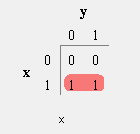
\includegraphics[width=0.3\textwidth]{recursos/Ejercicio3/mapas/mapa_a).png}
\end{center}

    \item Simplificación: \[ xy + x\overline{y} = x \]

    \item Circuito reducido:
\begin{center}
    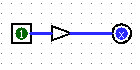
\includegraphics[width=0.4\textwidth]{recursos/Ejercicio3/circuito/circuito_a).png}
\end{center}
\end{itemize}

\subsection*{(b) $\overline{x}y + \overline{xy}$}

\begin{itemize}
    \item Mapa de Karnaugh:
\begin{center}
    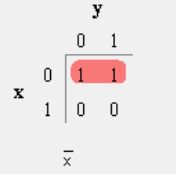
\includegraphics[width=0.4\textwidth]{recursos/Ejercicio3/mapas/mapa_b).png}
\end{center}

    \item Simplificación: \[ \overline{x}y + \overline{xy} = \overline{x} \]

    \item Circuito reducido:
\begin{center}
    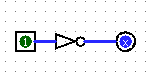
\includegraphics[width=0.3\textwidth]{recursos/Ejercicio3/circuito/circuito_b).png}
\end{center}
\end{itemize}

\subsection*{(c) $xyz + \overline{x}yz$}

\begin{itemize}
    \item Mapa de Karnaugh:
\begin{center}
    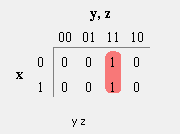
\includegraphics[width=0.4\textwidth]{recursos/Ejercicio3/mapas/mapa_c).png}
\end{center}

    \item Simplificación: \[ xyz + \overline{x}yz = yz \]

    \item Circuito reducido:
\begin{center}
    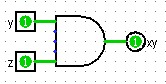
\includegraphics[width=0.3\textwidth]{recursos/Ejercicio3/circuito/circuito_c).png}
\end{center}
\end{itemize}

\subsection*{(d) $xy\overline{z} + x\overline{yz} + \overline{x}y\overline{z} + \overline{xyz}$}

\begin{itemize}
    \item Mapa de Karnaugh:
\begin{center}
    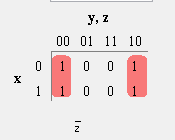
\includegraphics[width=0.4\textwidth]{recursos/Ejercicio3/mapas/mapa_d).png}
\end{center}

    \item Simplificación: \[ xy\overline{z} + x\overline{yz} + \overline{x}y\overline{z} + \overline{xyz} = \overline{z} \]

    \item Circuito reducido:
\begin{center}
    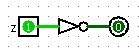
\includegraphics[width=0.3\textwidth]{recursos/Ejercicio3/circuito/circuito_d).png}
\end{center}
\end{itemize}

\subsection*{(e) $\overline{xy} + \overline{x}y + xy$}

\begin{itemize}
    \item Mapa de Karnaugh:
\begin{center}
    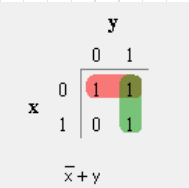
\includegraphics[width=0.3\textwidth]{recursos/Ejercicio3/mapas/mapa_e).png}
\end{center}

    \item Simplificación: \[ \overline{xy} + \overline{x}y + xy = \overline{x} + y \]

    \item Circuito reducido:
\begin{center}
    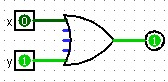
\includegraphics[width=0.3\textwidth]{recursos/Ejercicio3/circuito/circuito_e).png}
\end{center}
\end{itemize}

\subsection*{(f) $\overline{xy} + \overline{x}y + x + y$}

\begin{itemize}
    \item Mapa de Karnaugh:
\begin{center}
    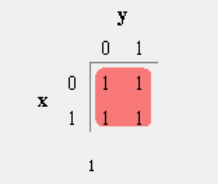
\includegraphics[width=0.3\textwidth]{recursos/Ejercicio3/mapas/mapa_f).png}
\end{center}

    \item Simplificación: \[ \overline{xy} + \overline{x}y + x + y = 1 \]

    \item Circuito reducido:
\begin{center}
    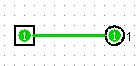
\includegraphics[width=0.3\textwidth]{recursos/Ejercicio3/circuito/circuito_f).png}

\end{center}
\end{itemize}


